\newpage
\section{Graf}

Foarte multe probleme pot fi descrise printr-o diagrama formata dintr-un set de puncte și linii care conecteaza anumite perechi de puncte.
De exemplu, punctele pot reprezenta o multime de persoane, iar liniile dintre ele relatii de rudenie, sau punctele pot centre de comunicare 
iar liniile fiind legăturile dintre ele. Se poate observa ca in astfel de diagrame importanta este pusa pe modul in care sunt conectate acele puncte,
aspectul fiind nesemnificativ. O abstractie matematica a situatilor de acest tip este conceptul de graf.\newline

Un graf este o structură formată din obiecte în care sunt puse în evidență legăturile dintre ele. 
Obiectele corespund unor abstracții matematice numite, într-un graf, noduri/vârfuri (puncte) și fiecare legătură 
dintre perechile de obiecte asociate se numește muchie (arc sau linie). 
De obicei, un graf este reprezentat în formă schematică ca un set/grup de puncte care reprezintă nodurile, iar aceste sunt unite două 
câte două de linii sau curbe care corespund mulțimii muchiilor. Muchiile pot fi orientate/directe sau neorientate/indirecte.\newline

Grafurile sunt numite astfel datorită reprezentării grafice, și datorită acestei reprezentări putem înțelege proprietățile lor mult mai ușor.
Nu există un mod unic de desenare a unui graf; pozițiile relative ale punctelor care reprezintă nodurile si ale liniilor care reprezintă muchiile nu au importanță.\newline


Din punct de vedere matematic un graf G este un triplet ordonat \((V(G),E(E),\psi_g)\) care conține un set nevid \(V(G)\) de noduri, un set \(E(G)\),
disjunct de \(V(G)\), de muchii și o funcție de incidență \(\psi_G\) care asociază fiecarei muchii din \(G\) o pereche neordonata (dar nu neaparat distinctă)
de noduri din \(G\). Dacă \(e\) este o muchie și avem nodurile \(u\) și \(v\) astfel încât \(\psi_G(e)=uv\), atunci se spune că \(e\) unește \(u\) și \(v\); 
nodurile \(u\) și \(v\) sunt numite capetele lui \(e\).\newline

Majoritatea definițiilor și conceptelor în teoria grafurilor sunt sugerate de reprezentarea grafică. Capetele unei muchii sunt incidente cu muchia, si vice versa. 
Doua noduri care sunt incidente cu o muchie comună sunt adiacente, la fel pentru doua muchii care sunt incidente cu un nod comun. O muchie cu capete identice se numeste bucla.\newline

Un graf este finit dacă ambele seturi, cel de noduri și cel de muchii, sunt finite. Totodata un graf cu un singur nod se numește trivial, iar restul grafurilor netriviale.
Un graf este simplu dacă nu are bucle și nu există doua muchii care unesc aceleași două noduri.\newline

Doua noduri \(u\) și \(v\) sunt conexe daca exista un drum \((u,v)\) in \(G\), adică o secvența de noduri unice legate prin muchii care începe cu \(u\) și se termină cu \(v\).
Conectivitatea este o relație de chivalență pe setul de noduri \(V\). Astfel există o partiționare a lui \(V\) un subseturi nevide \(V_1,V_2,...V_n\) astfel încăt nodurile \(u\) și \(v\)
sunt conexe dacă și numai daca sunt din același set \(V_i\). Subgrafurile \(G[V_1], G[V_2], ... , G[V_n]\) se numesc componente ale lui \(G\). Dacă \(G\) are o singură componentă, atunci
\(G\) este conex, altfel este neconex.\newline

Ordinul unui graf reprezinta numărul de noduri, notat cu \(|V|\). Mărimea unui graf este numărul de muchii \(|E|\).
Gradul unui nod este numărul de muchii care sunt incidente cu el.
Într-un graf de ordin \(n\), gradul maxim al oricărui nod este de \(n-1\), iar numărul maxim de muchii este \(n(n-1)/2\).

\subsection{Multigraf}

Un multigraf este o generalizare în care oricare doua noduri pot avea mai multe muchii între ele. Acele muchii sunt numite și muchii paralele sau muchii multiple.
Exista doua noțiuni distincte despre muchii paralele:\newline

\begin{itemize}
\item Muchii fără identitate: identitatea unei muchii ține de cele doua noduri de care aparține. 
În unele cazuri nevoia de a distinge muchii multiple dintre doua noduri poate lipsi, iar acele muchii sunt considerate ca o 
singura entitate.\newline
\item Muchii cu identitate: în acest caz fiecare muchie este considerată ca fiind o primitiva, la fel ca nodurile, 
iar în cazul în care intre doua noduri exista mai multe muchii, fiecare dintre ele este considerata fiind o entitate distinctă.\newline
\end{itemize}

Definiție matematică:\newline

\begin{itemize}
\item Multigraf neorientat, cu muchii fara identitate: 
\(G=(V,E)\) unde:
\begin{itemize}
    \item \(V\) este un set de noduri 
    \item \(E\) este un multiset de perechi de noduri, numite muchii.
\end{itemize}

    
\item Multigraf neorientat, cu muchii cu identitate:
\(G=(V,E,r)\), unde:
\begin{itemize}
    \item \(V\) este un set de noduri
    \item \(E\) este un set de muchii
    \item \(r : E → \{\{x,y\} : x, y \in V\}\)
\end{itemize}

\end{itemize}

\subsection{Graf planar}

Un graf planar este un graf care poate fi încorporat într-un plan, adică un graf care poate fi desenat astfel încât 
marginile sale sa se intersecteze doar în noduri. Cu alte cuvinte, muchiile grafului sa nu se suprapună.\newline

Matematicianul polonez Kazimierz Kuratowski a caractetizat idea de graf planar prin următoarea teoremă:\newline

Un graf finit este planar dacă și numai dacă nu conține un subgraf care este o subdiviziune a grafului complet \(K_5\) sau a grafului complet bipartit \(K_{3,3}\).
O subdiviziune a unui graf rezulta din inserarea a oricâte noduri într-o muchie.\newline

O alta modalitate de a descrie un graf planar este prin teorema lui Wagner, exprimată în legătura cu noțiunea de graf minor:\newline
 
Un graf finit este planar dacă și numai dacă nu conține grafurile \(K_5\) sau \(K_{3,3}\) ca graf minor. (figura \ref{fig:k5k33})
Un minor al unui graf rezulta prin contractarea unei muchii într-un nod, fiecare vecin al nodului original devenind vecin cu nodul nou.\newline

\begin{figure}[H]
    \begin{center}
        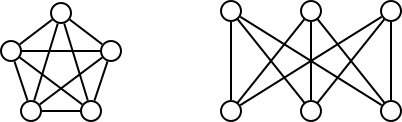
\includegraphics[scale=0.7]{imagini/graf/notplanar.png}        
    \end{center}
    \caption{Grafurile \(K_5\) si \(K_{3,3}\) \protect\footnotemark}
    \label{fig:k5k33}
\end{figure}

\footnotetext{\url{https://www.nomachetejuggling.com/assets/k33andk5.png}}

Alte criterii de planaritate:\newline
In practica este dificil sa folosim teorema lui Kuratowski pentru a decide într-un mod eficient dacă un graf este planar sau nu. 
Exista și alți algoritmi pentru rezolvarea acestei probleme, pentru un graf cu n noduri cu o complexitate de \(O(n)\).

Un graf simplu  cu \(v>=3\) noduri, \(e\) muchii și \(f\) fețe, trebuie sa îndeplinească următoarele condiții pentru a fi planar:
\begin{itemize}
    \item  \(e<=3v-6\)
    \item  dacă nu sunt cicluri de lungime \(3\), atunci \(e<=2v-4\) 
    \item  \(f<=2v-4\)
\end{itemize}

Formula lui Euler: \newline
Formula lui Euler afirmă că dacă un graf planar, finit, conectat, este desenat într-un plan și \(v\) este numărul de vârfuri, 
\(e\) este numărul de muchii și \(f\) este numărul de fețe (regiuni marcate de muchii , inclusiv regiunea exterioară, infinit de mare)
\[v-e+f=2\]

\begin{figure}[H]
    \begin{center}
        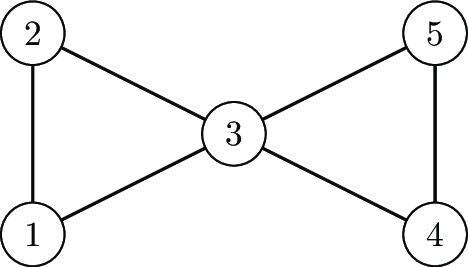
\includegraphics[scale=0.5]{imagini/graf/butterfly.png}
        \caption{Graf fluture \protect\footnotemark}
        \label{fig:fluture}
    \end{center}    
\end{figure}

\footnotetext{\url{https://www.researchgate.net/publication/328308578/figure/fig1/AS:682352216920065@1539696854150/The-butterfly-graph-five-nodes-with-two-node-pairs-connected-by-the-bridging-node-3.png}}

Ca o ilustrare, în graful fluture dat mai sus,(figura \ref{fig:fluture}) \(v = 5\), \(e = 6\) și \(f = 3\). În general, dacă proprietatea este valida 
pentru toate grafurile planare cu \(f\) fețe, orice modificare a grafului care ar crea o față suplimentară, graful 
fiind în continuare planar ar fi și \(v - e + f\) invariant. Din moment ce proprietatea este valid pentru toate grafurile 
cu \(f = 2\), prin inducție matematică este valabilă pentru toate cazurile. Formula lui Euler poate fi demonstrata și în 
modul următor: dacă graful nu este un arbore, șterge o muchie care completează un ciclu. Astfel scade atât e, cât și 
\(f\) cu unul, lăsând \(v - e + f\) constantă. Repetați până când graficul rămas este un arbore; copacii au \(v = e + 1\) și \(f = 1\), 
producând \(v - e + f = 2\).\newline

\subsection{Aplicare}

Grafurile pot fi folosite pentru modelarea relațiilor și proceselor într-un sistem fizic, biologic, 
social sau informatic. Multe probleme practice pot fi reprezentate prin grafuri. In domeniul informaticii 
grafurile pot fi folosite pentru a reprezenta rețele de comunicare, organizarea datelor, dispozitive computerizate, 
fluxul de calcul, etc. De exemplu și un site web poate fi reprezentat printr-un graf, paginile web fiind nodurile 
iar legăturile dintre ele, link-urile, fiind muchiile. O abordare similara poate fi proiectate pentru multe alte domenii, 
precum ingineria mecanica unde putem exprima relațiile dintre mai multe elemente mecanice printr-un graf. Dezvoltarea 
algoritmilor pentru a gestiona grafuri este, prin urmare, de interes major în domeniul informaticii.










